%!TEX root = ./template-skripsi.tex
%-------------------------------------------------------------------------------
%                            BAB II
%               KAJIAN TEORI
%-------------------------------------------------------------------------------

\chapter{KAJIAN PUSTAKA} 

\section{Definisi \emph{Search Engine}}

Mesin Pencari atau \emph{Search Engine} merupakan software yang digunakan untuk pencarian terhadap banyak situs web di internet berdasarkan input kata yang ditanyakan. \emph{Search Engine} memungkinkan pengguna untuk mencari situs web yang berkaitan dengan kata kunci ataupun pertanyaan yang diajukan oleh pengguna \citep{seymour2011history}.

Dalam penggunaannya, search engine hanyalah sebuah halaman situs website yang dapat diakses oleh pengguna yang perannya adalah mengumpulkan dan menampilkan hasil pencarian tersebut kepada user dengan tampilan yang menarik dan informatif \citep{seymour2011history}.

\section{Arsitektur \emph{Search Engine}}

Secara sederhana \emph{Search Engine} bekerja dengan menyimpan dan melakukan pengindeksan informasi-informasi dari situs web dan menyajikannya dalam bentuk yang dapat di mengerti oleh pengguna. Informasi dari halaman situs web didapatkan menggunakan program bernama \emph{Web crawler} yang mengunduh dan menyimpan informasi dari halaman situs web kedalam \emph{Database}. Setelah di simpan, infomasi akan dianalisis dan dipilih oleh program \emph{Indexer} \citep{lazuardithesis}.

\begin{figure}[H]
	\centering
	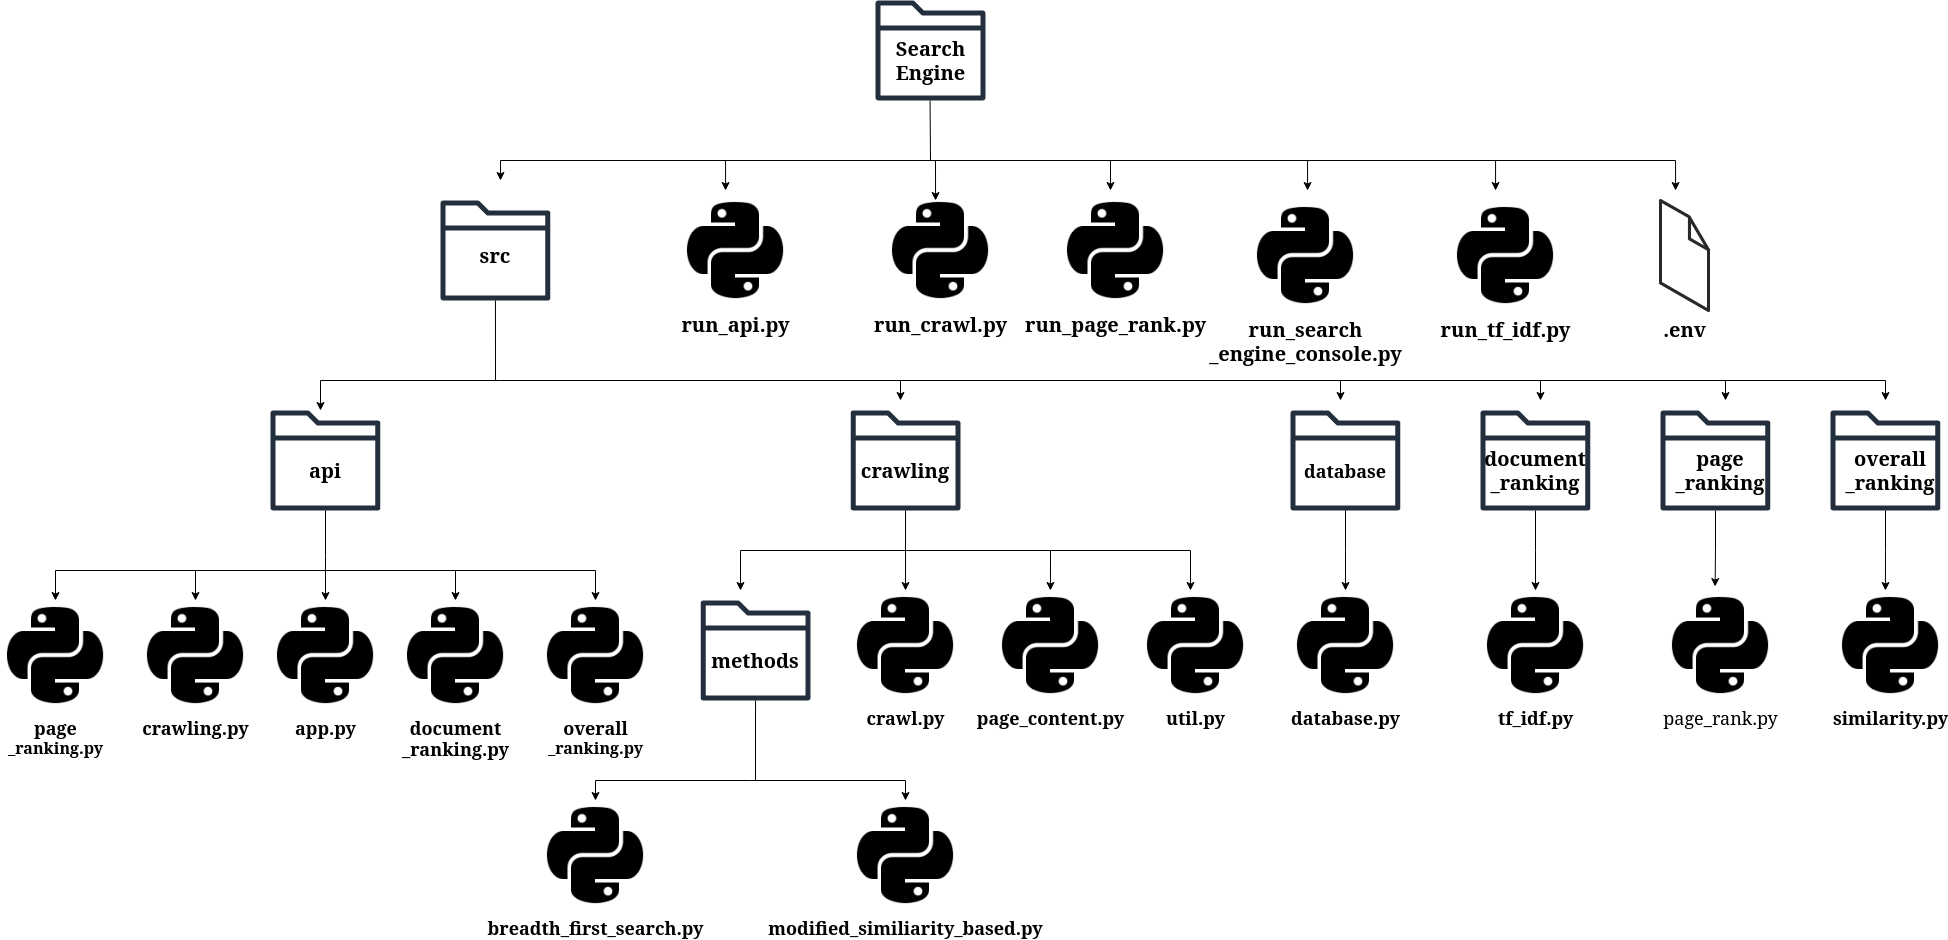
\includegraphics[keepaspectratio, width=14.5cm]{gambar/diagram-new.png}
  \caption{\emph{Struktur file \emph{search engine} Lazuardi} \citep{lazuardithesis}}
	\label{gambar:google_architecture}
\end{figure}

Proses \emph{crawling} dalam arsitektur \emph{Search engine} milik lazuard memiliki beberapa tahap, Tahap awal adalah \emph{crawler} akan mengakses \emph{origin url} yang disediakan dalam \emph{environment variable}. Untuk melakukan proses \emph{crawling}, perlu untuk menginisiasikan beberapa data yang akan digunakan dalam proses crawling seperti \emph{origin url} yang akan di akses, maksimum \emph{os threads} yang akan digunakan oleh crawler, dan durasi proses \emph{crawling}. Proses pertama yang dilakukan oleh \emph{crawler} setelah di inisiasi adalah dengan melakukan pengecekan ke \emph{database} apakah terdapat page yang sudah di \emph{crawl} atau belum, bila sudah maka crawler akan memulai proses \emph{crawling} dari page terakhir yang sebelumnya telah di \emph{parse}. Bila tidak, maka proses \emph{crawling} akan dimulai dari \emph{origin url}. List dari origin url akan dimasukkan kedalam \emph{queue} yang nantinya akan digunakan oleh proses \emph{Breadth First Search} dalam \emph{crawler}. Sebelum proses parse dilakukan data-data yang berhubungan dengan \emph{page} yang akan di \emph{parse} akan di insert kedalam database, seperti \emph{string url} dan duration \emph{parse}. Proses parsing page dilakukan menggunakan algoritma \emph{Breadth First Search}. Dalam menjalankan \emph{Breadth First Search}, setiap \emph{instance} \emph{page scrapper} dijalankan secara paralel didalam \emph{thread process}. \emph{Page scrapper} akan melakukan parsing tiap \emph{page} yang diakses dan mengambil beberapa bagian data dari  \emph{page} tersebut. Data yang parse dari \emph{page} merupakan data penting yang berisi inti sari dari \emph{page} tersebut dan data lain yang akan mendukung proses \emph{crawling} dan proses-proses selanjutnya dalam arsitektur \emph{search engine}, beberapa data yang diambil oleh \emph{scrapper} adalah \emph{article body} dari \emph{html page}, \emph{meta description} dari \emph{page}, \emph{meta keyword}, \emph{css page style} dari page, \emph{script} yang di \emph{embedded} dalam page, \emph{list}, \emph{form}, \emph{table}, \emph{image} dalam \emph{page}, dan \emph{hyperlink} yang ada di \emph{page} tersebut. Data-data yang telah dikumpulkan tersebut akan di masukkan ke dalam \emph{database} \citep{lazuardithesis}.

Dalam proses \emph{crawling} setiap kali \emph{page scrapper} selesai dalam menjelajahi dan melakukan \emph{parsing} dalam satu page, \emph{page scrapper} akan memasukkan url list yang di dapat dari dalam page kedalam \emph{queue}. Agar proses penambahan link kedalam queue tidak terganggu, penambahan \emph{queue} dilakukan secara \emph{syncronous} menggunakan lock. \emph{Url list} yang disimpan di dalam \emph{queue} ini nantinya akan di akses oleh \emph{page scrapper} lain. Proses ini akan berlanjut terus secara paralel dan pengaksesan tiap-tiap url dilakukan menggunakan algoritma \emph{breadth first search} \citep{lazuardithesis}.

\subsection{\emph{Breadth First Search}}

Untuk menjelajahi \emph{url list} yang ada di dalam \emph{queue} \emph{crawler} menggunakan algoritma \emph{breadth first search}, algoritma ini pada dasarnya merupakan algoritma untuk menjelajahi \emph{graph} dalam suatu \emph{tree}. Dalam penerapannya di dalam arsitektur \emph{search engine} milik lazuardi \emph{breadth first search} dimanfaatkan dalam proses pemilihan url yang akan diakses dalam setiap iterasi proses \emph{page scrapping} \citep{lazuardithesis}. Dalam menjelajahi \emph{tree}, algoritma ini menggunakan struktur data \emph{queue} untuk menyimpan informasi tentang \emph{node} yang akan dijelajahi selanjutnya dan \emph{stack} untuk menyimpan informasi mengenai \emph{node} yang telah di jelajahi. Metode \emph{breadth first search} memungkinkan untuk \emph{crawler} memprioritaskan penjelajahan \emph{url} yang telah dimasukkan ke dalam \emph{queue} terlebih dahulu, hal ini menjamin agar setiap tingkatan \emph{node} sudah dijelajahi sebelum lanjut ke tingkat \emph{node} selanjutnya \citep{cormen2009introduction}.

\begin{algorithm}[H]
	\caption{\emph{BFS($G,s$)} \citep{cormen2009introduction}}
	\label{algoritma_bfs}
	\begin{algorithmic}[1]
		\For{each vertex $u \in G.V - \{s\}$}
		\State $ u.color =$ WHITE
		\State $ u.d = \infty$
		\State $ u.\pi =$ NIL
		\EndFor
		\State $ s.color = $ GRAY
		\State $s.d = 0$
		\State $s.\pi = NIL$
		\State $Q = \infty$
		\State ENQUEUE($Q,s$)
		\While{$Q\not=\emptyset$}
		\State $u =$ DEQUEUE(Q)
		\For{each $v \in G.Adj[u]$}
		\If{$v.color ==$ WHITE}
		\State $v.color ==$ GRAY
		\State $v.d = u.d +1$
		\State $v.\pi = u$
		\State ENQUEUE($Q, v$)
		\State $v.color ==$ BLACK
		\EndIf
		\EndFor
		\EndWhile
	\end{algorithmic}
\end{algorithm}

Dalam arsitektur \emph{search engine} milik Lazuardi algoritma \emph{breadth first search} didefinisikan di dalam \emph{class BreadthFirstSearch}, \emph{class} ini terletak di dalam file \url{breadth_first_search.py}. Di dalam penerapan algoritma \emph{breadth first search} pada arsitektur \emph{search engine} milik lazuardi proses jalannya algoritma \emph{breadth first search} dibagi menjadi dua tahap, proses yang berjalan di dalam \emph{main thread} dan proses yang berjalan di dalam individual \emph{thread} yang sudah di \emph{spawn}. Contoh penerapan \emph{breadth first search} dalam arsitektur lazuardi dapat dilihat pada \ref{gambar:bfs_python} \citep{lazuardithesis}.

\begin{figure}[H]
	\centering
	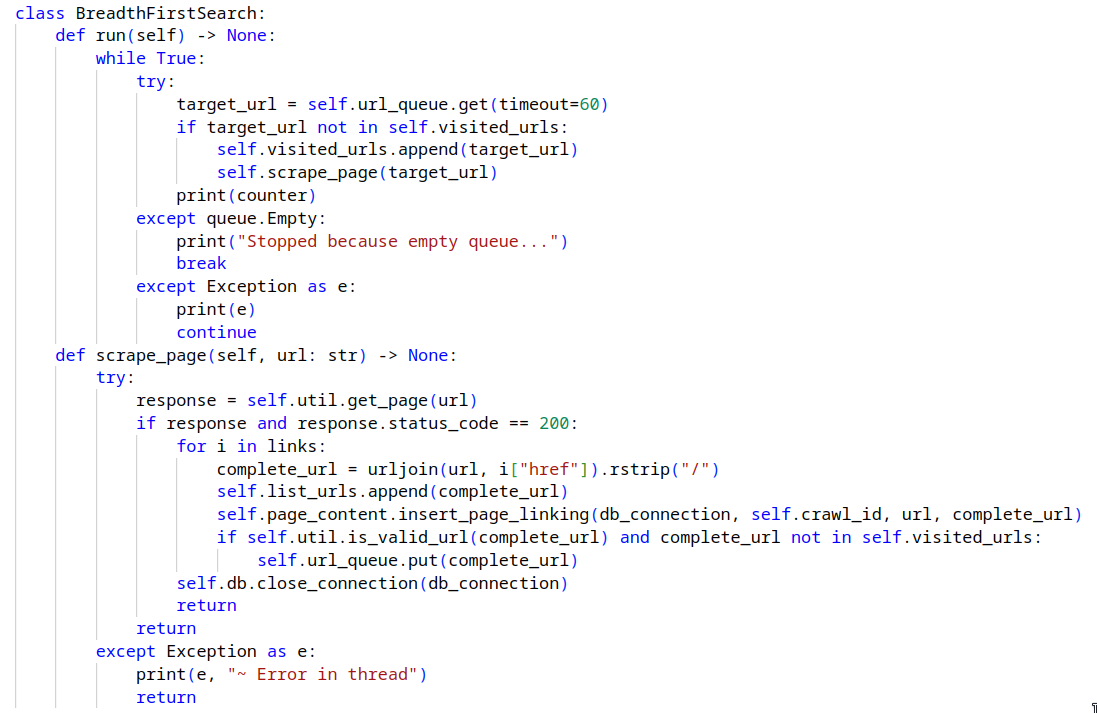
\includegraphics[keepaspectratio, width=15cm]{gambar/bfs-python.png}
  \caption{Algoritma \emph{breadth first search} dalam arsitektur lazuardi \citep{lazuardithesis}}
	\label{gambar:bfs_python} 
\end{figure}

Jalannya \emph{breadth first search} di arsitektur milik lazuardi dimulai dengan mengambil list \emph{url} dari \emph{queue} yang ada ke dalam variabel \emph{target\_url}, setelah itu dilakukan pengecekkan terhadap \emph{url} tersebut pada \emph{visited\_url} yang ada didalam \emph{stack}, bila \emph{url} itu belum pernah dikunjungin maka \emph{url} tersebut akan di marked sebagai \emph{visited url}. \emph{Url} yang telah di tandai akan di proses di dalam fungsi \emph{scrape\_page}, di dalam fungsi ini \emph{url} yang diterima akan di akses dan di \emph{parse}. Salah satu target pencarian dari proses \emph{parsing} page adalah \emph{url} page lain yang ditanam di dalam \emph{page} tersebut, \emph{url} tersebut akan di masukkan kedalam \emph{array} dan \emph{queue crawler} \citep{lazuardithesis}. Algoritma ini menggunakan struktur data \emph{queue} yang menggunakan prinsip \emph{First In First Out}, hal ini menyebabkan data atau dalam skenario ini \emph{url} yang terlebih dahulu diambil oleh crawler merupakan \emph{url} yang dimasukkan lebih awal, mekanisme ini mendukung agar algoritma dapat menjelajahi tiap-tiap level \emph{tree} secara menyeluruh sebelum pindah ke level \emph{tree} yang lebih dalam \citep{cormen2009introduction}. 

\begin{figure}[H]
	\centering
	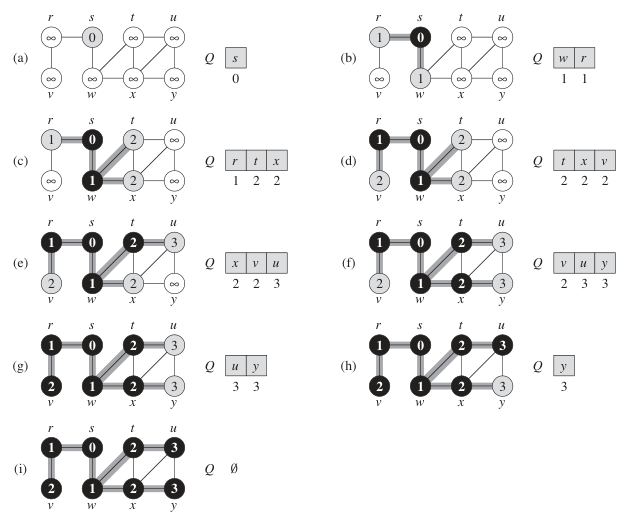
\includegraphics[keepaspectratio, width=10cm]{gambar/bfs-diagram.png}
  \caption{\emph{Diagram alur algoritma \emph{breadth first search} \citep{cormen2009introduction}}}
	\label{gambar:bfs_diagram} 
\end{figure}

\subsection{\emph{Threading}}

Untuk menjalankan algoritma \emph{breadth first search} proses \emph{page scrapping} secara efisien, arsitektur \emph{search engine} lazuradi memanfaatkan proses \emph{multi-thread}. Thread merupakan bagian terkecil dari suatu proses yang berjalan secara berurutan yang dapat dijalankan dan dikelola oleh \emph{cpu scheduler} dan pada dasarnya hanya terdapat satu proses yang dapat berjalan dalam satu thread \citep{operatingsystemconcept}. Arsitektur \emph{search engine} milik lazuardi memanfaatkan \emph{thread} untuk mengisolasi setiap proses \emph{page scrapping} dan menjalankannya secara paralel, hal ini memungkinkan untuk tiap-tiap instance dari \emph{page scrapper} untuk berjalan secara independen dalam melakukan penjelajahan dan \emph{parsing} dari halaman \emph{website}.

\begin{figure}[H]
	\centering
	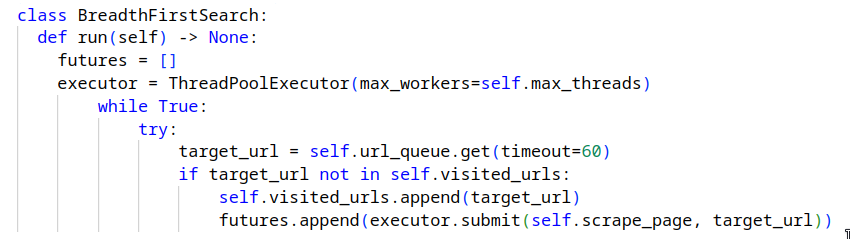
\includegraphics[keepaspectratio, width=15cm]{gambar/threading-python.png}
  \caption{Algoritma \emph{multi threading} dalam arsitektur lazuardi \citep{lazuardithesis}}
	\label{gambar:threading_python} 
\end{figure}
 
Proses \emph{threading} dalam arsitektur \emph{search engine} lazuardi dimulai dengan pengalokasian jumlah \emph{thread} maksimum yang dapat di gunakan oleh proses \emph{page scrapping}, jumlah maksimum thread ini dapat diatur sesuai dengan kapasitas \emph{cpu} mesin dan berapa banyak halaman \emph{web} yang akan di \emph{crawl}, proses pengalokasian jumlah maksimum \emph{thread} ini dilakukan menggunakan \emph{ThreadPoolExecutor}. \emph{ThreadPoolExecutor} merupakan \emph{class} dari \emph{python} yang berfungsi untuk mengatur pengalokasian beberapa jumlah \emph{thread} secara otomatis, ini mempermudah proses alokasi sumber daya \emph{thread} untuk proses yang ditentukan dengan jumlah \emph{thread} yang telah ditentukan. \emph{Thread pool} yang telah diinisiasi selanjutnya digunakan untuk menjalankan fungsi \emph{scrape\_page} yang sudah didefinisikan sebelumnya, hal ini agar setiap jalannya fungsionalitas \emph{page scrapper} berjalan diatas satu \emph{thread process}. Dengan menggunakan \emph{thread} proses \emph{scraping} dapat berjalan secara \emph{asyncronous} dan penjelajahan tiap-tiap halaman \emph{website} berjalan lebih cepat \citep{lazuardithesis}.

\subsection{\emph{Parsing} Halaman \emph{website} dan penyimpanan data}

Dalam jalannya proses algoritma \emph{breadth first search} yang sudah dijelaskan sebelumnya terdapat satu proses yang dinamakan \emph{page scrapping}. Proses ini bertujuan untuk mengekstraksi data penting dari halaman \emph{website} yang sedang di kunjungi oleh \emph{crawler}, data - data ini dikumpulkan ini lah yang nantinya akan digunakan untuk proses - proses selanjutnya dalam alur arsitektur \emph{search engine} milik lazuardi. Dalam arsitektur \emph{search engine} milik lazuardi proses ini di lakukan dengan menggunakan bantuan library \emph{beautifulsoup4} \citep{lazuardithesis}. Dalam implementasi arsitektur \emph{search engine} milik lazuardi proses \emph{page scrapping} dilakukan didalam setiap satu \emph{thread} yang telah dibuat sebelumnya dan satu proses \emph{page scrapping} akan berjalan pada satu halaman \emph{website}, hal ini dilakukan untuk menjamin jalannya proses \emph{page scrapping} berjalan dengan cepat. Informasi yang di ambil dari proses \emph{page scrapping} akan di bagi kedalam beberapa kategori, tujuannya untuk menjaga konsistensi data dan mempermudah proses selanjutnya dalam melakukan pengambilan data \citep{lazuardithesis}.

  \begin{center}
    \begin{longtable}{ |p{1cm}|p{3cm}|p{7cm}| }
      \caption{\emph{HTML Tag} dari halaman \emph{web} yang di ambil oleh \emph{crawler} \citep{lazuardithesis}} \\

      \hline \textbf{no}.& \textbf{tag}& \textbf{deskripsi} \\ \hline
      \endfirsthead

      \hline \textbf{no}.& \textbf{tag}& \textbf{deskripsi} \\ \hline
      \endhead

      \hline \multicolumn{3}{r}{{Dilanjutkan pada halaman berikutnya}} \\
      \endfoot

      \hline \hline
      \endlastfoot

      1& \emph{body/article}& konten utama \\ \hline
      2& \emph{meta description}& Deskripsi singkat dari halaman web \\ \hline
      3& \emph{meta keyword}& Kata kunci yang merepresentasikan isi halaman web \\ \hline
      4& \emph{style}& \emph{css style} dalam suatu halaman web \\ \hline
      5& \emph{list}& isi dari \emph{list} yang terdapat dalam halaman web \\ \hline
      6& \emph{form}& form dan input yang terdapat dalam halaman web \\ \hline
      7& \emph{table}& kumpulan elemen \emph{table} dalam halaman web \\ \hline
      8& \emph{image}& kumpulan \emph{url} yang mengarah pada gambar di halaman web \\ \hline
      9& \emph{outgoing link}& kumpulan \emph{url} referensi yang mengarah pada halaman web lain \\ \hline
    \end{longtable}
  \end{center}

  Data-data yang telah dikelompokkan ini selanjutnya akan dimasukkan ke dalam \emph{database} yang sudah disiapkan. Struktur data dari \emph{database} akan mencerminkan permbagian kategori data yang didapatkan seperti Tabel 2.1. Gambar \ref{gambar:lazuardy_database} merupakan struktur \emph{database} yang digunakan oleh arsitektur \emph{search engine} lazuardy \citep{lazuardithesis}.

\begin{figure}[H]
	\centering
	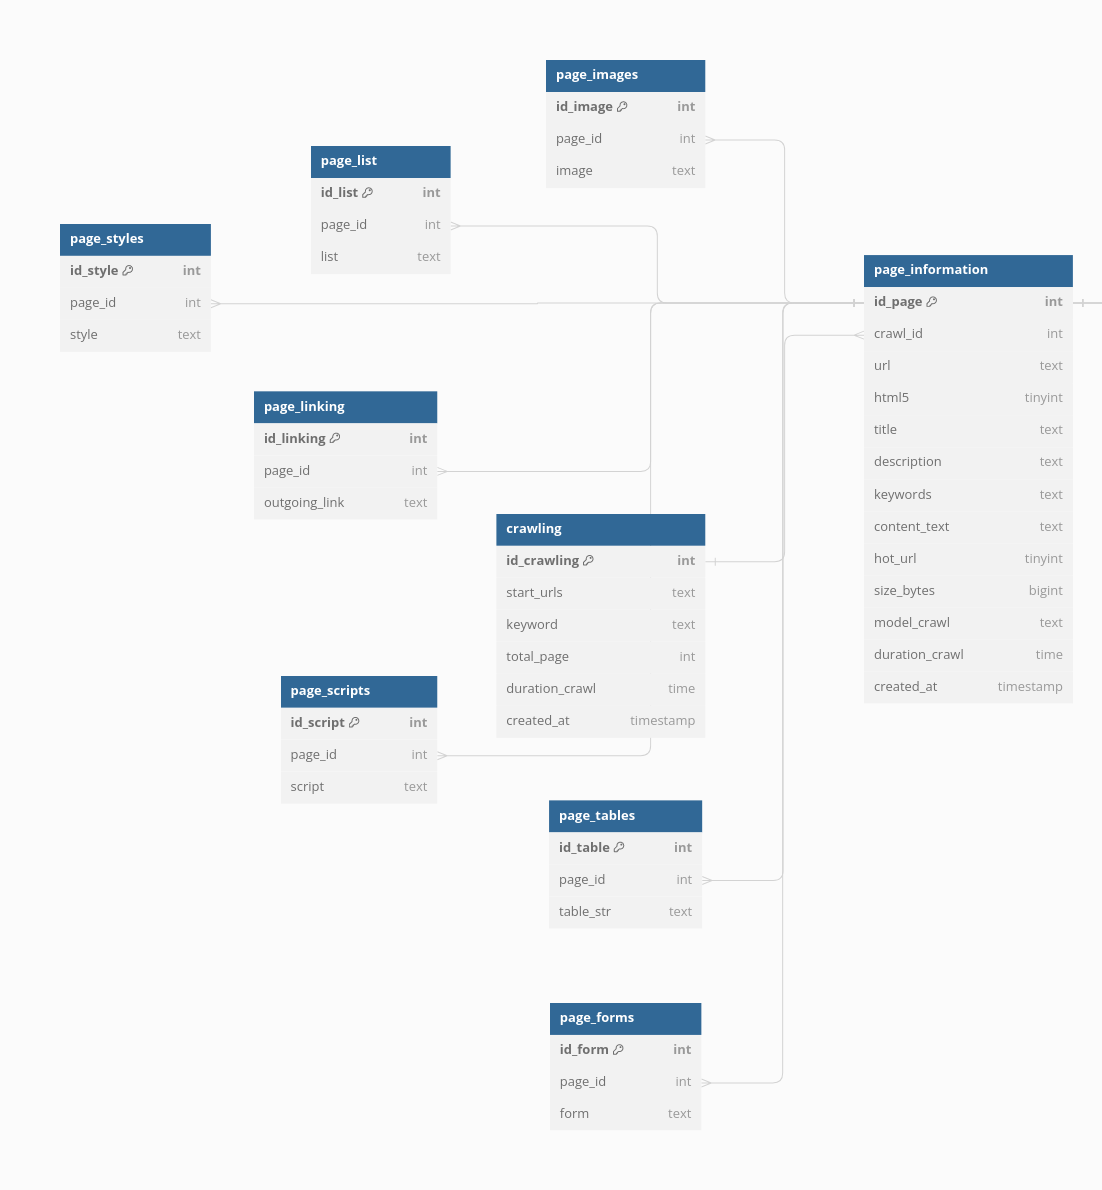
\includegraphics[keepaspectratio, width=14.5cm]{gambar/crawler-erd.png}
  \caption{\emph{Entity Relations Diagram} database lazuardi \citep{lazuardithesis}}
	\label{gambar:lazuardy_database}
\end{figure}

\subsection{\emph{Library} dalam arsitektur \emph{search engine} Lazuardy}

Arsitektur \emph{search engine} milik lazuardy dikembangkan menggunakan platform bahasa pemograman \emph{python} dengan menggunakan \emph{runtime cpython} versi 3.0. Untuk menjalankan fungsionalitas \emph{search engine} terdapat penggunaan berbagai \emph{standard library} dan \emph{third-pary library} dalam menjalankan proses tertentu seperti pengambilan data dari halaman web sampai penyimpanan data ke dalam \emph{database}. \emph{Standard library} dari \emph{python} yang digunakan dalam arsitektur ini adalah \emph{queue}, \emph{time}, \emph{threading}, \emph{os}, \emph{regex} dan, \emph{request} \citep{lazuardithesis}.

  \begin{center}
    \begin{longtable}{ |p{1cm}|p{4cm}|p{5cm}| }
      \caption{Daftar \emph{library} yang digunakan dalam arsitektur \emph{search engine} milik lazuardy \citep{lazuardithesis}} \\ \hline

      \multicolumn{3}{|c|}{Daftar \emph{library} \emph{third party}} \\ \hline
      \endfirsthead

      \hline \multicolumn{3}{|c|}{Daftar \emph{library} \emph{third party}} \\ \hline
      \endhead

      \hline \multicolumn{3}{r}{{Dilanjutkan pada halaman berikutnya}} \\
      \endfoot

      % Last footer without next page indication
      \hline \hline
      \endlastfoot

      No.& Nama \emph{library}& Fungsi \\ \hline
      1.& \emph{beautifulsoup4}& Parsing menyusun \emph{language tree} untuk mengambil informasi \\ \hline
      2.& \emph{requests}& Melakukan \emph{request} untuk mengunduh halaman \emph{website} \\ \hline
      3.& \emph{pandas}& Melakukan interaksi dengan matriks \\ \hline
      4.& \emph{pymysql}& \emph{Interface} untuk melakukan operasi \emph{query} \\ \hline
      5.& \emph{python-dotenv}& Mengambil data dari \emph{environtment variable} \\ \hline
      6.& \emph{psutil}& Melakukan \emph{monitoring} dan pengambilan informasi dari \emph{process} \emph{python} yang berjalan \\ \hline
      7.& \emph{scikit-learn}& Membuat model perhitungan \emph{TF-IDF} \\ \hline
      8.& \emph{numpy}& Melakukan perhitungan matematika kompleks \\ \hline
      9.& \emph{pdoc3}& Penulisan Dokumentasi \\ \hline
      10.& \emph{flask}& Penyediaan \emph{API} \emph{server} untuk antarmuka operasi \emph{search engine} \\ \hline
    \end{longtable}
  \end{center}

\section{\emph{Process dan Threads}}

Pada awalnya komputer generasi awal hanya bisa menjalankan satu program pada satu waktu, program ini memiliki akses penuh terhadap semua \emph{resources} pada komputer. Keterbatasan komputer generasi awal ini membuat hal yang dapat dilakukan di komputer menjadi sangat terbatas, berbeda komputer generasi awal komputer generasi sekarang dapat menjalankan beberapa program secara bersamaan. Hal ini didukung dengan arsitektur komputer yang \emph{multi-core} dan kapasitas \emph{memory} yang lebih besar. Dengan banyaknya penggunaan komputer dengan jumlah \emph{core} yang banyak, mekanisme agar komputer dapat menjalankan beberapa program sekaligus semakin dibutuhkan. Komputer \emph{modern} memiliki mekanisme yang dapat digunakan agar beberapa program dapat di muat kedalam \emph{memory} dan dijalankan secara bersamaan, terdapat dua metode yang dapat mendukung jalannya mekansime ini, yaitu \emph{process} dan \emph{threads} \citep{operatingsystemconcept}.

\subsection{\emph{Process}}

\emph{Process} pada dasarnya adalah \emph{program} yang sedang dijalankan oleh komputer, \emph{program} pada sendirinya hanya file pasif yang berisi instruksi - instruksi yang perlu dijalankan oleh komputer. Instruksi tersebut yang menjadi satu \emph{instance} dari \emph{process}. \emph{Process} mengakses data yang diperlukan untuk proses komputasi dari \emph{virtual memory}, data di dalam memory ini bersifat sementara dan disimpan sebagai \emph{cache}. \emph{Memory} yang dapat diakses oleh \emph{process} memiliki susunan tertentu yang terbagi menjadi beberapa bagian.
\begin{figure}[H]
	\centering
	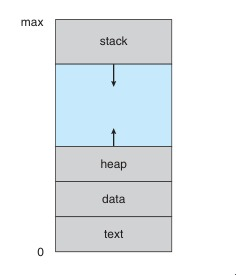
\includegraphics[keepaspectratio, width=6cm]{gambar/memory-layout.jpeg}
  \caption{Susunan bagian dari \emph{virtual memory} \citep{operatingsystemconcept}}
	\label{gambar:memory_layout}
\end{figure}

Dari gambar \ref{gambar:memory_layout} dapat dilihat bahwa susunan \emph{vitual memory} yang dapat diakses oleh \emph{process} yang berjalan terbagi menjadi beberapa bagian yang dibagi berdasarkan jenis data yang disimpan dan tingkat alamat dari data tersebut dalam \emph{memory} \citep{operatingsystemconcept}. Bagian-bagian dalam \emph{virtual memory} adalah,

\begin{enumerate}
  \item \emph{Text}. Data yang berisi kode yang dijalankan
  \item \emph{Data}. Data yang berisi variabel global dalam kode
  \item \emph{Heap}. Sejumlah Ukuran \emph{memory} yang dialkokasikan secara dinamis oleh program saat program sedang berjalan atau \emph{runtime}
  \item \emph{Stack}. Penyimpanan data sementara yang disediakan saat pemanggilan fungsi dalam kode.
\end{enumerate}

Ukuran dari bagian \emph{text} dan \emph{data} dalam memory adalah tetap, sedangkan ukuran \emph{heap} dan \emph{stack} dapat bertambah dan berkurang secara dinamis saat \emph{process} sedang berjalan. Walaupun \emph{program} atau kode dapat membuat dua \emph{process} yang berbeda, setiap \emph{process} tersebut memiliki blok \emph{virtual memory} masing-masing dengan data dalam bagian \emph{text} yang sama dan bagian lain seperti \emph{data}, \emph{heap}, dan \emph{stack} yang berbeda sesuai dengan instruksi yang diajalankan pada setiap \emph{process} \citep{operatingsystemconcept}.

Saat \emph{process} berjalan, \emph{process} akan mengubah \emph{state}. \emph{State} adalah indikasi status dari \emph{process} terkait yang sedang berjalan. State dari \emph{process} akan berubah ketika terdapat operasi yang dilakukan terhadap \emph{process} terkait, nama dan alur dari perubahan \emph{state} ini berbeda di setiap \emph{operating system} tetapi konsep dari \emph{process state} ini dapat ditemukan di semua \emph{operating system} \citep{operatingsystemconcept}.

\begin{figure}[H]
	\centering
	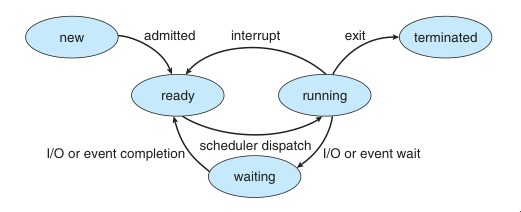
\includegraphics[keepaspectratio, width=12cm]{gambar/state-process.jpeg}
  \caption{Alur perubahan dari \emph{process state} \citep{operatingsystemconcept}}
	\label{gambar:state_process_flow}
\end{figure}

Dari gambar \ref{gambar:state_process_flow} dapat dilihat alur perubahan dari \emph{process state} dan \emph{event} apa yang dapat memicu perubahan \emph{process state} tersebut. Perlu diketahui gambar \ref{gambar:state_process_flow} tidak menampilkan perubahan \emph{process state} yang spesifik dari \emph{operating system} tertentu, tetapi \emph{state} yang dari figur tersebut dapat ditemui di seluruh \emph{operating system} \citep{operatingsystemconcept}. \emph{State} yang ada di gambar \ref{gambar:state_process_flow} adalah,

\begin{enumerate}
  \item{\emph{New}. \emph{Process} baru yang dibuat}
  \item{\emph{Running}. Instruksi yang sedang di eksekusi}
  \item{\emph{Waiting}. \emph{Process} yang sedang menunggu \emph{trigger event}}
  \item{\emph{Ready}. \emph{Process} yang menunggu alokasi \emph{processor}}
\end{enumerate}

\subsection{\emph{Inter-process Communication}}

Beberapa \emph{process} yang dijalankan secara bersamaan oleh \emph{operating system} dapat dibagi menjadi dua kategori \emph{process} yang berjalan sendiri dan tidak berkaitan dengan \emph{process} lain, dan \emph{process} yang jalannya berkaitan dengan \emph{process} lain. \emph{Process} yang mekanismenya berkaitan dengan \emph{process} lain perlu strategi dan mekanisme dalam berbagi data dengan \emph{process}, hal ini dapat disebut  dengan \emph{inter-process communication} \citep{operatingsystemconcept}.

Terdapat 2 mekanisme dasar \emph{inter-process communication} yaitu mekanisme \emph{shared memory} dan \emph{message passing}. Dalam mekanisme \emph{shared memory} terdapat bagian dari \emph{virtual memory} yang di digunakan secara bersamaan oleh 2 \emph{process} yang berkaitan, dengan metode ini kedua \emph{process} akan menulis dan mengambil data dari bagian \emph{virtual memory} yang sama. Dalam metode \emph{message passing} data yang dikomunikasikan melalui pertukaran pesan antara dua \emph{process} \citep{operatingsystemconcept}. 

\begin{figure}[H]
  \centering
	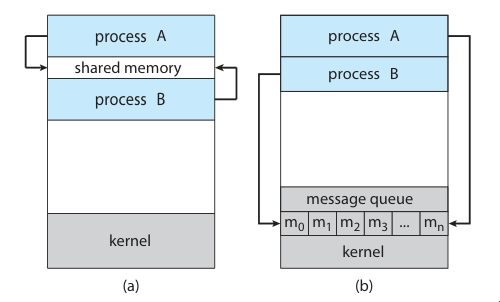
\includegraphics[keepaspectratio, width=12cm]{gambar/ipc_models.png}
  \caption{Metode komunikasi antar \emph{process}. (a) \emph{Shared memory}. (b) \emph{Message passing} \citep{operatingsystemconcept}}
	\label{gambar:ipc_models}
\end{figure}

Selain 2 metode yang sudah dijelaskan sebelumnya juga terdapat metode \emph{inter-process communication} yang lebih berfokus pada komunikasi pada sistem \emph{client-server}, salah satu metodenya adalah \emph{socket}. \emph{Socket} secara definisi merupakan metode komunikasi antar proses yang dikirimkan dengan format tertentu kepada alamat tertentu. \emph{Socket} sendiri terbagi menjadi dua jenis, yaitu \emph{network socket} yang dapat digunakan dua perangkat berbeda untuk berkomunikasi dengan perantara jaringan internet dan \emph{UNIX domain socket} yang hanya dapat digunakan oleh komunikasi antar proses dalam perangkat yang sama dengan sistem operasi yang bersifat \emph{POSIX compliant} \citep{operatingsystemconcept}.

\subsection{\emph{Threads}}

\emph{Process} dapat di jelaskan sebagai \emph{program} yang dijalankan dalam satu \emph{threads} yang berjalan, contoh dari konsep ini adalah ketika \emph{program} pengolah kata sedang dijalankan instruksi-instruksi yang ada pada \emph{program} dijalankan secara berurutan dalam satu \emph{thread} yang berjalan. \emph{Thread} memungkinkan untuk \emph{process} untuk menjalankan satu \emph{instruction} dalam satu waktu dan membuat jalan dari keseluruhan \emph{instruction} dalam \emph{program} untuk berjalan secara berurutan. Dalam \emph{operating system} modern konsep dari \emph{thread} ini ditingkatkan sehinggan satu \emph{process} dapat menjalankan beberapa \emph{thread} secara bersamaaan sehingga lebih dari satu \emph{instruksi} dapat dijalankan secara bersamaan \citep{operatingsystemconcept}. 

\begin{figure}[H]
  \centering
	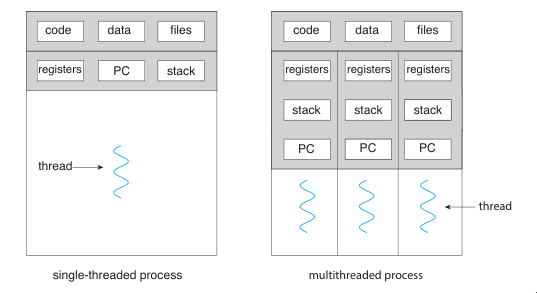
\includegraphics[keepaspectratio, width=12cm]{gambar/thread_process.png}
  \caption{\emph{Process} dengan satu \emph{thread} dan lebih dari satu \emph{thread} \citep{operatingsystemconcept}}
	\label{gambar:thread_process}
\end{figure}

Dalam gambar \ref{gambar:thread_process} terlihat bahwa beberapa \emph{thread} yang berjalan secara bersamaan dalam satu \emph{process} yang sama pada dasarnya berbagi \emph{resources} seperti \emph{virtual memory} yang sama. Hal ini memungkinkan dalam jalannya satu \emph{program} beberapa instruksi dengan \emph{performance cost} yang besar untuk dilankan secara bersamaan dengan proses sinkronisasi data yang lebih mulus, selain itu proses locking antar \emph{thread} akan lebih mudah dikelola dengan adanya \emph{virtual memory} yang sama antar \emph{thread} \citep{operatingsystemconcept}. 

Mekanisme pembuatan dan jalannya \emph{thread} bergantung dengan sistem operasi yang digunakan dalam perangkat. Dalam sistem operasi \emph{windows} aplikasi berjalan diatas \emph{process} dan tiap \emph{process} terdiri dari satu atau lebih \emph{thread}, \emph{windows} menggunakan strategi \emph{one to one mapping} dalam manajemen \emph{thread}-nya dimana \emph{thread} dibagi menjadi dua jenis yaitu \emph{thread} yang berjalan di dalam \emph{user space} dan \emph{kernel space}. Setiap \emph{thread} dalam \emph{user space} dipetakan ke \emph{thread kernel} yang terkait. Dalam \emph{windows} pembagian jenis \emph{thread} terlihat dengan jelas dan memiliki struktur data yang pasti. Terdapat 3 struktur data \emph{thread} dalam windows yaitu \emph{ETHREAD} atau \emph{executive thread block}, \emph{KTHREAD} atau \emph{kernel thread block}, dan \emph{TEB} atau \emph{therad environment block} \citep{operatingsystemconcept}.

\begin{figure}[H]
  \centering
	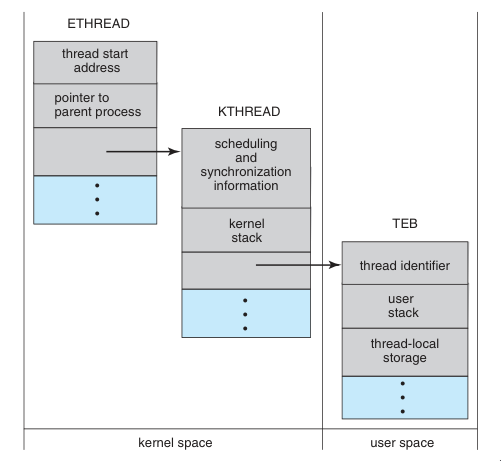
\includegraphics[keepaspectratio, width=10cm]{gambar/windows-thread.png}
  \caption{Struktur data dari \emph{windows thread} \citep{operatingsystemconcept}}
	\label{gambar:windows_thread}
\end{figure}

Berbeda dengan \emph{window}, pembagian jenis \emph{thread} dalam sistem operasi \emph{linux} tidak terlihat dengan jelas. \emph{Linux} menyediakan dua \emph{system call} untuk berinteraksi dengan pembuatan \emph{process} dan \emph{thread} yaitu \emph{fork()} dan \emph{clone()}, tetapi \emph{linux} tidak membedakan secara spesifik antara \emph{thread} dan \emph{process}. Perbedaan antara \emph{thread} dan \emph{process} dalam \emph{linux} terlihat dari seberapa banyak pembagian data yang terjadi diantara tiap-tiap \emph{task}, pembagian ini dideklarasikan ketika \emph{system call} dipanggil dengan menambakan \emph{flags} tambahan \citep{operatingsystemconcept}.

\begin{figure}[H]
  \centering
	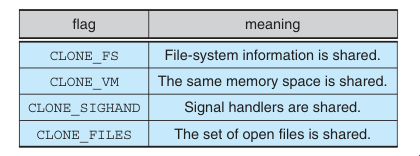
\includegraphics[keepaspectratio, width=10cm]{gambar/linux-thread.png}
  \caption{\emph{flags} yang dapat dipanggil \emph{clone()} \citep{operatingsystemconcept}}
	\label{gambar:linux_thread}
\end{figure}

Gambar \ref{gambar:linux_thread} merupakan \emph{flags} yang dapat dipanggil ketika memanngil \emph{system call} \emph{clone()}, setiap \emph{flags} memiliki tinkat pembagian \emph{resources} yang berbeda \citep{operatingsystemconcept}.

\section{\emph{Rust Programming Language}}

\emph{Rust programming language} merupakan bahasa pemograman level sistem dengan penekanan desain bahasa yang aman, dapat bekerja dengan konkuren dan cepat. \emph{Rust} sama seperti dengan bahasa pemograman sistem yang lain seperti \emph{C} atau \emph{C++} mengkompilasi kodenya menjadi \emph{machine code}, hal ini memberika dorongan kinerja yang lebih cepat terhadap hasil \emph{program} terhadap bahasa lain yang menggunakan mekanisme \emph{interpretation} seperti \emph{javascript} dan \emph{python} atau terhadap bahasa pemograman \emph{java} yang menggunakan \emph{virtual machine} untuk mentranslasi kode nya \citep{rustbook}. Layak nya bahasa pemograman sistem yang lain \emph{rust} menyediakan \emph{interface} untuk berinteraksi dengan abstraksi level rendah pada komputer seperti manajemen \emph{memory}, pengaturan terhadapa konkurensi dengan \emph{process} dan \emph{thread} dan akses terhadap \emph{API} dari \emph{operating system}. \emph{Rust} juga membawa konsep baru ke dalam dunia pemograman sistem dalam melakukan manajemen alokasi \emph{memory} dinamis di sistem, berbeda dengan bahasa pemograman \emph{C} dan \emph{C++} yang melakukan alokasi dan pelepasan \emph{space} pada memory bila sudah tidak digunakan secara manual \emph{rust} menggunakan sistem \emph{variable ownership} dan \emph{borrowing} ini memungkinkan \emph{rust} untuk tidak menggunakan \emph{garbage collector} dalam \emph{runtime} tetapi tetap menjaga keamanan \emph{memory}-nya \citep{rustbook}.

\subsection{Konsep Semantik Dari \emph{Ownership}}

Ketika \emph{program} ingin mengalokasikan ruang dalam \emph{memory} untuk menyimpan data yang dinamis bahasa pemograman harus mampu melakukan dua hal yaitu, mekanisme untuk mengalokasikan ruang dalam \emph{memory} untuk menyimpan data saat \emph{runtime} dan yang kedua adalah cara untuk melepas \emph{memory} tersebut kembali ke \emph{operating system} ketika data teresebut sudah tidak digunakan \citep{rustbook}. Bahasa pemograman dengan abstraksi level tinggi seperti \emph{python}, \emph{javascript}, \emph{go} dan \emph{java} menggunakan mekanisme \emph{garbage collection}, mekanisme ini memungkian agar \emph{program} untuk mengalokasikan ruang pada \emph{memory} ketika dibutuhkan dan melepas \emph{memory} ketika tidak dibutuhkan secara otomatis. Mekanisme \emph{garbage collection} dilakukan pada saat \emph{runtime} sehingga mempengaruhi performa dan waktu eksekusi dari program, ini membuat program yang dijalankan dengan mekanisme \emph{garbage collection} berjalan lebih lambat. Bahasa dengan abstraksi yang lebih rendah seperti \emph{C} dan \emph{C++} melakukan alokasi dan pelepasan ruang pada \emph{memory} secara manual, hal ini membuat \emph{program} yang dibuat rentan terhadap penggunaan \emph{memory} yang berlebihan atau data yang tidak valid ketika diakses. \emph{Rust} menggunakan sistem yang berbeda dari bahasa pemograman lain dalam mekanisme manajemen \emph{memory}, yaitu \emph{ownership} dan \emph{borowing} \citep{rustbook}

\emph{Ownership} adalah konsep manajemen \emph{memory} dalam \emph{rust} dengan konsep utama kepemilikan data oleh \emph{variable} \citep{rustbook}. Dalam mekanisme \emph{ownership} terdapat tiga aturan utama yaitu,

\begin{enumerate}
  \item{Setiap nilai atau \emph{value} memiliki \emph{variable} yang menjadi pemiliknya yang disebut \emph{owner}}
  \item{Setiap nilai hanya dapat memiliki \emph{owner} dalam satu waktu}
  \item{Ketika \emph{owner} dari nilai tersebut keluar dari cakupan, nilai nya akan dihapus}
\end{enumerate}

\emph{Rust} secara otomatis mengembalikan ruang yang dipakai di \emph{memory} oleh \emph{variable} yang sudah keluar dari jangkauan program. Keluar dari Jangkauan atau \emph{out of scope} adalah kondisi ketika \emph{variable} sudah tidak dapat digunakan atau di-akses \citep{rustbook}.
\begin{figure}[H]
  \centering
	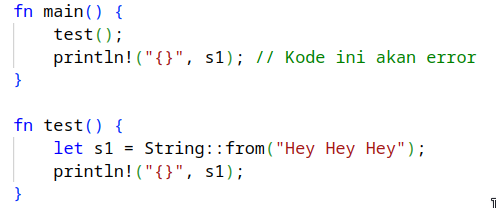
\includegraphics[keepaspectratio, width=12cm]{gambar/rust-scope.png}
  \caption{Scope dalam \emph{rust} \citep{rustbook}}
	\label{gambar:rust-scope}
\end{figure}

Dalam gambar \ref{gambar:rust-scope} terdapat dua \emph{function}, \emph{test()} dan \emph{main()}. Dalam fungsi \emph{test()} terdapat deklarasi \emph{variable} \emph{s1} berupa \emph{string}, data di-dalam \emph{s1} disimpan di-dalam \emph{heap} dan \emph{owner}-nya adalah \emph{s1}. Variabel \emph{s1} memiliki jangkauan hanya didalam \emph{test()}, ini artinya \emph{s1} tidak dapat di akses di luar fungsi \emph{test()} dan ini menjelaskan mengapa kode pada gambar \ref{gambar:rust-scope} akan error. Berbeda dengan bahasa pemograman lain, ketika variabel yang data-nya di simpan dalam \emph{heap} memiliki sifat-sifat yang unik dikarenakan pengaruh \emph{ownership} \citep{rustbook}.

\begin{figure}[H]
  \centering
	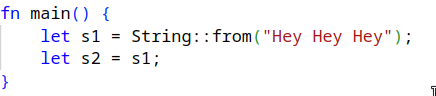
\includegraphics[keepaspectratio, width=12cm]{gambar/moving-data.png}
  \caption{Memindahkan data dari variabel \emph{s1} ke \emph{s2} \citep{rustbook}}
	\label{gambar:rust-data-transfer}
\end{figure}

\begin{figure}[H]
  \centering
	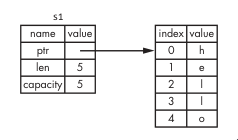
\includegraphics[keepaspectratio, width=7cm]{gambar/single-s1-memory.png}
  \caption{Representasi penyimpanan data dalam variabel \emph{s1} dalam \emph{memory} \citep{rustbook}}
	\label{gambar:single-memory-representation}
\end{figure}

\begin{figure}[H]
  \centering
	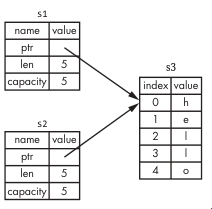
\includegraphics[keepaspectratio, width=7cm]{gambar/double-s1-s2-memory.png}
  \caption{Representasi penyimpanan data yang sama dalam dua variabel \emph{s1} dan \emph{s2} dalam \emph{memory} \citep{rustbook}}
	\label{gambar:double-memory-representation}
\end{figure}

Di kode dalam gambar \ref{gambar:rust-data-transfer} terlihat seperti data dari \emph{s1} di-\emph{copy} dan disimpan kedalam variabel \emph{s2}. Gambar \ref{gambar:single-memory-representation} merupakan representasi dalam \emph{memory} dari string yang disimpan dalam variabel \emph{s1}, tabel \emph{s1} dan tabel \emph{s2} merupakan data yang disimpan di dalam \emph{stack} dan berisi 3 komponen yaitu panjang dari \emph{string} tersebut, kapasitas maksimal dari \emph{string}, dan \emph{pointer} yang menunjuk ke lokasi di \emph{memory} yang menyimpan isi dari \emph{string} tersebut \citep{rustbook}. Tabel \emph{s3} merupakan isi sebenarnya dari \emph{string} tersebut yang disimpan di dalam \emph{heap}. Ketika variabel \emph{s1} disalin dan disimpan ke variabel baru, yang sebenarnya terjadi adalah data yang disalin hanya data dalam \emph{stack} saja dan data dalam variabel baru akan memiliki \emph{pointer} yang menunjuk ke lokasi \emph{heap} yang sama dengan data asli nya seperti yang terlihat di gambar \ref{gambar:double-memory-representation}. Ketika variabel keluar dari jangkauan \emph{program} \emph{rust} secara otomatis akan menghapus data variabel tersebut yang terdapat di dalam \emph{heap}, bila dalam skenario kode \ref{gambar:rust-data-transfer} kedua variabel \emph{s1} dan \emph{s2} keluar dari jangkauan program maka kedua variabel itu akan mencoba untuk menghapus data yang sama dalam \emph{memory}, hal ini disebut dengan nama \emph{double free error} yang merupakan permasalahan keamanan \emph{memory} yang \emph{rust} mencoba untuk tangani \citep{rustbook}.

\begin{figure}[H]
  \centering
	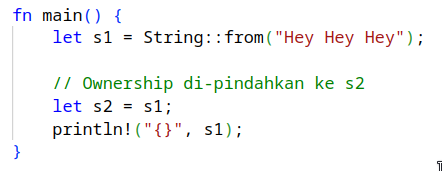
\includegraphics[keepaspectratio, width=12cm]{gambar/ownership-transfer.png}
  \caption{Memindahkan ownership dari variabel \emph{s1} ke \emph{s2} \citep{rustbook}}
	\label{gambar:rust-ownership-transfer}
\end{figure}

Untuk menghindari permasalahan keamanan yang terkait dengan \emph{double free error}, dalam kode \ref{gambar:rust-data-transfer} yang terjadi bukan hanya sekedar proses penyalinan \emph{memory} yang telah di alokasikan. Alih-alih hanya melakukan penyalinan, \emph{rust} akan menganggap \emph{s1} tidak lagi valid dan maka dari itu \emph{memory} yang berkaitan dengan \emph{s1} tidak perlu di hapus ketika \emph{s1} keluar dari jangkauan \emph{program} akibatnya, variabel \emph{s1} bila diakses setelah data-nya dipindahkan tidak akan berhasil \citep{rustbook}. Seperti yang terlihat di kode dalam gambar \ref{gambar:rust-ownership-transfer}, ketika \emph{s1} di-\emph{print} tidak akan berhasil.

Untuk melakukan proses penyalinan data dalam \emph{heap} yang tidak berbenturan dengan \emph{ownership}, \emph{rust} menyediakan metode \emph{clone}. \emph{Clone} merupakan metode penyalinan data yang berbasis dari konsep \emph{deep copy} ini berarti ketika metode ini dipanggil variabel kedua tidak hanya menyalin data dalam \emph{stack} saja namun juga menyalin data dalam \emph{heap} dari variabel tersebut, ini membuat metode \emph{clone} cocok untuk menyalin variabel yang data-nya disimpan didalam \emph{heap} seperti \emph{string} dan \emph{slice}. Kekurangan dari \emph{clone} adalah karena data dalam \emph{heap} juga disalin, jumlah \emph{memory} yang digunakan menjadi besar.\citep{rustbook}

\begin{figure}[H]
  \centering
	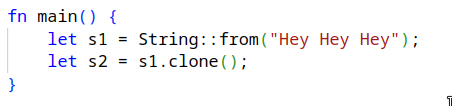
\includegraphics[keepaspectratio, width=12cm]{gambar/rust-clone-method.png}
  \caption{Penyalinan data \emph{s1} ke \emph{s2} \citep{rustbook}}
	\label{gambar:rust-clone-method}
\end{figure}

Ketika variabel diteruskan ke dalam \emph{function} secara semantik hal yang terjadi serupa dengan inisiasi data kedalam variabel. Meneruskan variabel kedalam \emph{function} akan memindahkan atau menyalin data seperti inisiasi variabel. Dalam kode \ref{gambar:rust-function-ownership} dapat dilihat contoh penggunaan \emph{function} dalam berinteraksi dengan \emph{ownership} dalam variabel \citep{rustbook}.

\begin{figure}[H]
  \centering
	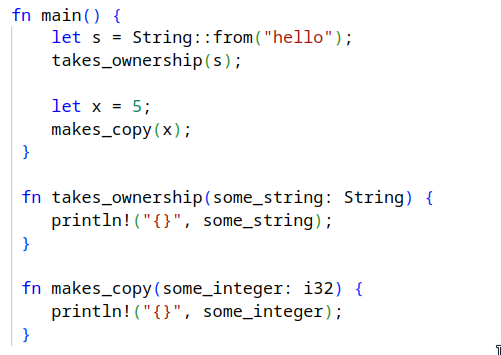
\includegraphics[keepaspectratio, width=12cm]{gambar/function-ownership.png}
  \caption{Penggunaan \emph{function} dengan \emph{ownership} \citep{rustbook}}
	\label{gambar:rust-function-ownership}
\end{figure}

Dalam kode \ref{gambar:rust-function-ownership} ketika \emph{function} mengambil parameter suatu variabel yang datanya berada di \emph{heap} dan variabel nya keluar cakupan dalam \emph{function} tersebut maka data-nya akan di hapus. Berbeda dengan ketika data yang tersimpan dalam \emph{stack} yang di lempar kedalam \emph{parameter} suatu \emph{function}, ketika variabel tersebut keluar jangkauan dalam \emph{function} tersebut tidak akan membuat variabel-nya terhapus \citep{rustbook}.

\begin{figure}[H]
  \centering
	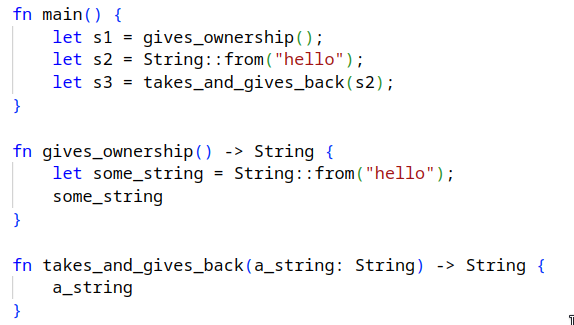
\includegraphics[keepaspectratio, width=12cm]{gambar/return-value-scope.png}
  \caption{Penggunaan \emph{function} dengan \emph{ownership} \citep{rustbook}}
	\label{gambar:rust-ownership-return}
\end{figure}

Dalam kode \ref{gambar:rust-ownership-return} dapat dilihat bahwa data dari \emph{return value} suatu \emph{function} juga dapat di berikan \emph{ownership}-nya kepada variabel yang menampungnya, ini berarti variabel \emph{some\_string} keluar jangkauan saat \emph{function}-nya selesai tetapi dikarenakan data dari \emph{some\_string} si pindahkan saat pemanggilan \emph{function} dalam bentuk \emph{return value},  \emph{ownership} dari data tersebut di berikan ke \emph{s1} \citep{rustbook}.

\subsection{Konsep Semantik Dari \emph{Borrowing} dan \emph{Reference}}

\begin{figure}[H]
  \centering
	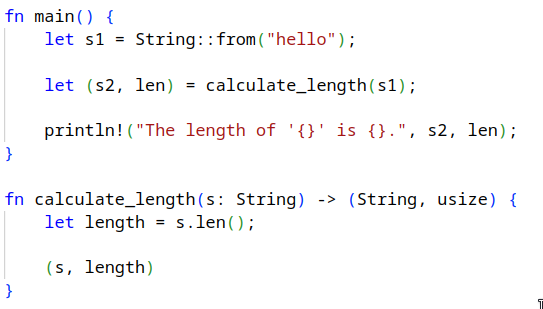
\includegraphics[keepaspectratio, width=12cm]{gambar/print-string-and-length.png}
  \caption{Program untuk mencari panjang dari \emph{string} dalam \emph{rust} \citep{rustbook}}
	\label{gambar:rust-length-string}
\end{figure}

Dalam kode \ref{gambar:rust-length-string} fungsi \emph{calculate\_length} berfungsi untuk menghitung panjang dari string, dalam fungsi tersebut terdapat dua \emph{return value} dikarenakan fungsi tersebut ketika menerima parameter \emph{string} \emph{s1} secara otomatis \emph{ownership} dari variabel tersebut diberikan ke \emph{calculate\_length}. Agar kode \ref{gambar:rust-length-string} dapat mengakses kembali nilai \emph{string} dalam \emph{s1} fungsi \emph{calculate\_length} perlu juga memberikan \emph{return value} berupa \emph{string} tersebut, keterbatasan penggunaan variabel yang berinteraksi dengan parameter suatu fungsi membuat fungsi \emph{calculate\_length} menjadi kompleks. Untuk mengindari kompleksitas tambahan yang diasosiasikan dengan pemindahan \emph{ownership} kepada fungsi lain perlu digunakan \emph{reference} atau \emph{borrowing} \citep{rustbook}. 

\emph{Referece} merupakan sebuah \emph{pointer} yang menunjuk kepada alamat dari data asli tersebut dalam \emph{memory}. Ketika suatu variabel dibuat \emph{reference}-nya, \emph{ownership} dari data tersebut masih terikat dengan variabel asalnya dan \emph{reference} tersebut hanya berisi alamat variabel asal-nya saja \citep{rustbook}. 

\begin{figure}[H]
  \centering
  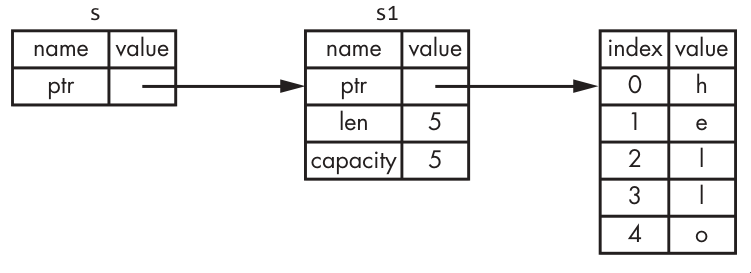
\includegraphics[keepaspectratio, width=12cm]{gambar/reference-memory.png}
  \caption{Representasi penggunaan \emph{referece} dalam \emph{memory} \citep{rustbook}}
  \label{gambar:reference-memory-ilust}
\end{figure}

Dari kode \ref{gambar:reference-memory-ilust} dapat dilihat bahwa variabel \emph{s} yang merupakan \emph{reference} dari \emph{s1}, maka \emph{s} hanya menyimpan data mengenai alamat dari variabel \emph{s1} saja dan sisa dari data disimpan di \emph{s1} \citep{rustbook}.

\begin{figure}[H]
  \centering
  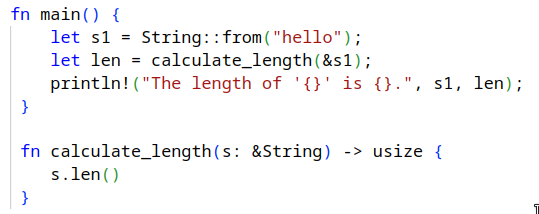
\includegraphics[keepaspectratio, width=12cm]{gambar/reference-rust-code.png}
  \caption{Semantik penggunaan \emph{reference} dalam \emph{rust} \citep{rustbook}}
  \label{gambar:reference-code-rust}
\end{figure}

Kode dalam gambar \ref{gambar:reference-code-rust} merupakan contoh penggunaan \emph{reference} dalam \emph{rust} yang direpresentasikan dalam gambar \ref{gambar:reference-memory-ilust}. Dikarenakan \emph{ownership} dari data tidak berpindah saat \emph{reference} digunakan, maka penggunaaan \emph{reference} dalam parameter fungsi disebut dengan nama \emph{borrowing}. \emph{Borrowing} adalah aksi ketika fungsi meminjam data dari variabel menggunakan \emph{reference} sehingga \emph{ownership} dari data tersebut akan dikembalikan ke variabel yang memiliki \emph{ownership} dari data tersebut. Dapat dilihat dari kode dalam gambar \ref{gambar:reference-memory-ilust} ketika \emph{reference} dari \emph{s1} dimasukkan ke dalam fungsi \emph{calculate\_length}, \emph{ownership} dari data-nya tidak di pindahkan ke variabel \emph{s} tetapi fungsi tetap dapat melakukan operasi terhadap data tersebut dan ketika fungsi \emph{calculate\_length} selesai dijalankan data dari variabel tersebut tidak dihapus.  \citep{rustbook}.

\subsection{Semantik Struktur Data dalam \emph{Rust}}

\emph{Struct} atau \emph{Structure} merupakan tipe data khusus yang dapat mengelompokkan dan menamakan lebih dari satu tipe data yang berkaitan, \emph{struct} digunakan sebagai metode untuk menyimpan struktur data yang lebih kompleks dengan komposisi data yang bervariasi.\citep{rustbook}

\begin{figure}[H]
  \centering
  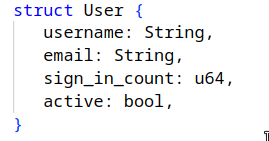
\includegraphics[keepaspectratio, width=7cm]{gambar/struct-declare-rust.png}
  \caption{\emph{Struct} yang mendefinisikan data \emph{user} \citep{rustbook}}
  \label{gambar:struct-definition-rust}
\end{figure}

Kode \ref{gambar:struct-definition-rust} merupakan mekanisme dalam mendefinisikan \emph{struct} dalam \emph{rust}, \emph{struct} itu diberi nama \emph{user} dan berisi data-data seperti \emph{username}, \emph{email}, \emph{sign in count}, dan \emph{active} dengan tipe data yang berbeda-beda. \emph{Struct} hanya mendefinisikan rancangan dari tipe data khusus yang akan dibuat dan selama data ini belum diinisiasi belum ada ruang dalam \emph{memory} dinamis yang dialokasikan \citep{rustbook}.

\begin{figure}[H]
  \centering
  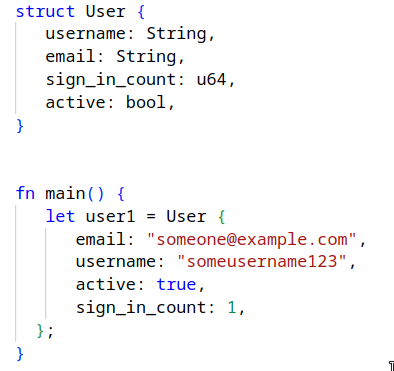
\includegraphics[keepaspectratio, width=9cm]{gambar/rust-object-declaration.png}
  \caption{Deklarasi objek dalam \emph{rust} \citep{rustbook}}
  \label{gambar:object-declaration-rust}
\end{figure}

Untuk menggunakan struktur data yang didefinisikan dalam \emph{struct} diperlukan untuk membuat objek atau \emph{instance} dari \emph{struct} tersebut, kode dalam gambar \ref{gambar:object-declaration-rust} variabel \emph{user1} merupakan objek atau \emph{instance} yang dibuat berdasarkan \emph{struct} \emph{user}. Dalam pembuatan objek \emph{user1}, data-data atau \emph{fields} yang menyusun objek tersebut diisi dengan nilai-nilai tertentu seperti data \emph{username} yang diisi dengan nilai \emph{someusername123}. Objek yang telah dibuat berdasarkan desain dari \emph{struct} dapat digunakan sebagai tempat untuk menyimpan data yang kompleks, dan data-data tersebut dapat diakses ataupun di modifikasi saat jalannya program \citep{rustbook}.

\begin{figure}[H]
  \centering
  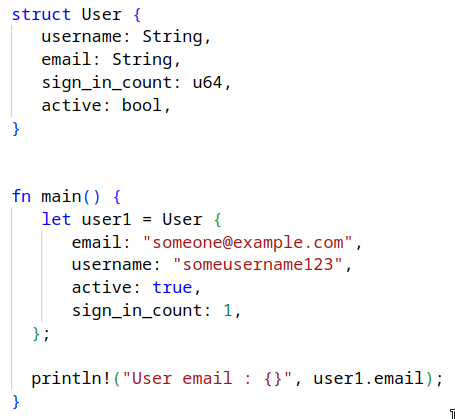
\includegraphics[keepaspectratio, width=9cm]{gambar/rust-accessing-attributes.png}
  \caption{Mengakses atribut kelas di \emph{Rust} \citep{rustbook}}
  \label{gambar:attributes-accesing-rust}
\end{figure}

\emph{Attributes} atau data yang disimpan di dalam \emph{struct} dapat diakses dengan memanggil objek tersebut seperti yang ditunjukan pada kode dalam gambar \ref{gambar:attributes-accesing-rust}. Dengan memanggil nama objek \emph{user1} yang diinisasi menggunakan sesuai dengan \emph{struct} \emph{User} dan mengakses \emph{attributes} email, data dari \emph{attributes} email dapat diakses dan diubah secara langsung \citep{rustbook}.

Selain menggunakan \emph{struct}, \emph{rust} juga menyediakan cara lain dalam menyimpan data kompleks yaitu \emph{enum}. \emph{Enum} atau \emph{enumerates} merupakan struktur data untuk meyimpan data yang merupakan kemungkinan dari pilihan kumpulan data, perbedaan yang paling mencolok antara \emph{struct} dan \emph{enum} adalah \emph{struct} menyimpan data yang terkait dan dapat diibaratkan dengan kata dan sedangkan \emph{enum} menyimpan data terkait yang merupakan pilihan yang dapat diibaratkan dengan kata atau.\citep{rustbook}

\begin{figure}[H]
  \centering
  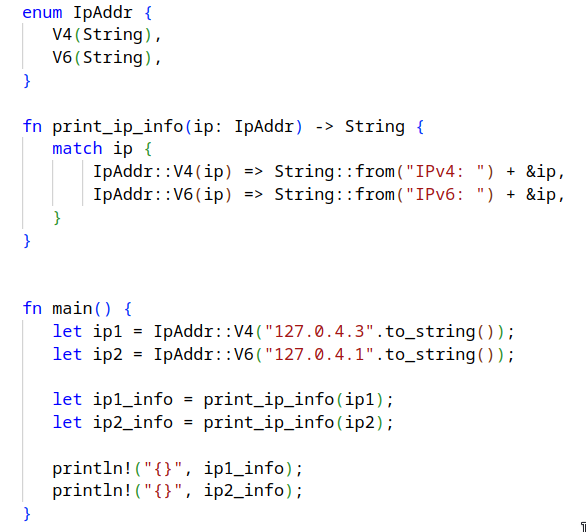
\includegraphics[keepaspectratio, width=12cm]{gambar/rust-enum-operations.png}
  \caption{Operasi yang memanfaatkan \emph{enum} pada \emph{rust} \citep{rustbook}}
  \label{gambar:enum-operations-rust}
\end{figure}

Dalam kode \ref{gambar:enum-operations-rust}, pendeklarasian \emph{enum} \emph{IpAddr} dilakukan pertama kali. Sama seperti \emph{struct}, \emph{enum} \emph{IpAddr} hanyalah struktur data rancangan dan data baru di deklarasikan di fungsi \emph{main} saat pembuatan variabel \emph{ip1}. Perbedaan \emph{enum} dengan \emph{struct} dapat dilihat dari isi \emph{enum} yang dideklarasikan, dimana saat deklarasi \emph{enum} variabel yang dibuat harus memilih diantara pilihan attribut yang ada \citep{rustbook}.

\begin{figure}[H]
  \centering
  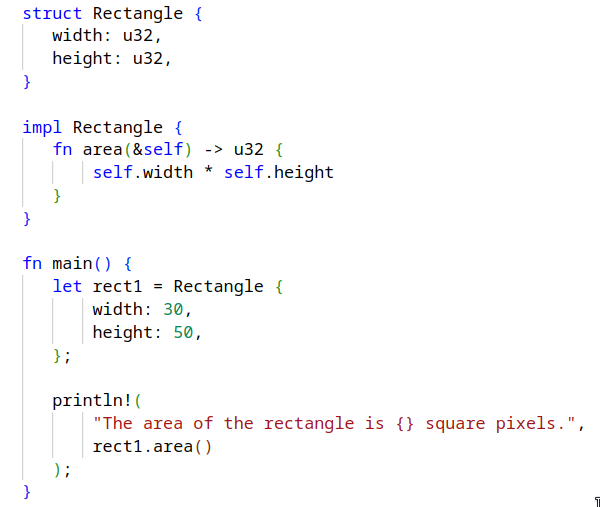
\includegraphics[keepaspectratio, width=12cm]{gambar/rust-struct-method.png}
  \caption{\emph{Method} dalam \emph{rust} \citep{rustbook}}
  \label{gambar:method-struct-rust}
\end{figure}

Metode yang disarankan untuk operasi yang mengubah nilai dari data yang disimpan dalam \emph{struct} dan \emph{enum} adalah menggunakan \emph{method}. \emph{Method} pada dasarnya serupa dengan \emph{function}, perbedaan-nya adalah \emph{method} merupakan \emph{function} yang di-definisikan dalam konteks \emph{struct} atau \emph{enum}. \emph{Method} dapat dengan bebas memodifikasi semua data yang disimpan di dalam \emph{struct} atau \emph{enum}. Seperti kode dalam gambar \ref{gambar:method-struct-rust}, parameter pertama dari \emph{method} adalah \emph{self} yang merepresentasikan objek dari \emph{struct} atau \emph{enum} yang terkait \citep{rustbook}.

